\documentclass[a4paper,12pt,french] {article}

\usepackage[sujet]{../../Style}

\fancyhead[L]{15/11/2021}
\fancyhead[C]{\textbf{DS2 : Vecteurs du plan}}
\fancyhead[R]{\seconde 12}

\renewcommand{\baselinestretch}{1.25}

\usetikzlibrary{decorations,decorations.markings,calc}

\begin{document}

\rem{L'usage de la calculatrice est autorisé. La propreté et l'orthographe seront prises en compte. Tout le devoir peut être fait sur cette feuille.}

Nom: \hfill Prénom: \hfill \

\begin{exercice}
Calculer \underline{en détaillant}:
\vspace{2mm}

\begin{center}
\begin{minipage}{0.9\textwidth}
$A=\left( \frac {-3} 4 \right)^3 \times \left( \frac {-3} 4 \right)^2$ \hfill $B=\frac {\left(2^5\right)^7 \times 2^{-13}} {2^{12}} $ \hfill $C=\frac { 15^5 \times 5^2 } {3^2 \times 5^3}$
\end{minipage}
\end{center}
\vspace{70mm}
\end{exercice}

\begin{exercice} \
%%%%% A la base le graphique était vertical, enlever les deux options pour avoir l'original ( il faudra refaire les labels )
\compo[0.38]
{
En utilisant le repère ci-contre:
\begin{enumerate}
\item Tracer deux représentants du vecteur $\vv {AB}$, l'un d'origine $D$, l'autre d'extrémité $C$.
\item Placer $M$, l'image de $C$ par la translation de vecteur $\vv {DB}$.
\item Placer $N$, l'image de $C$ par la translation de vecteur $\vv {DC}$.
\end{enumerate}
}
{
\begin{center}
\vspace{-5mm}
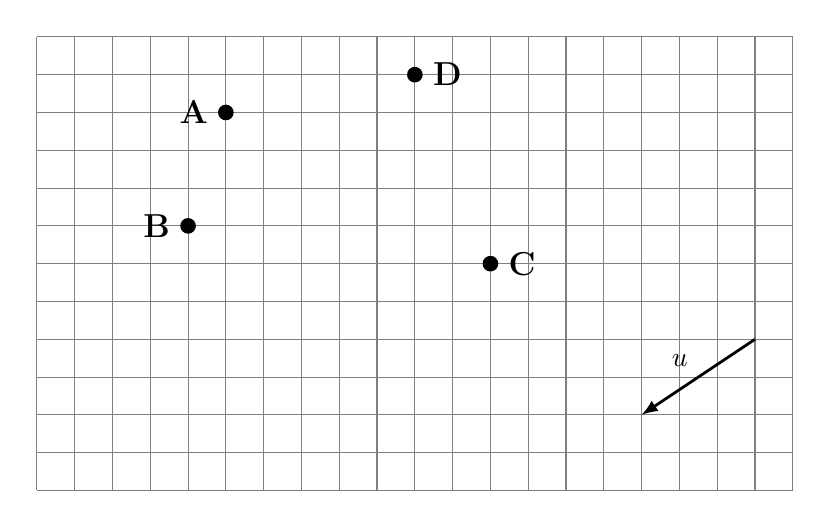
\begin{tikzpicture}[scale=0.48,rotate=-90,yscale=-1]
\node[draw=none] (liminf) at (1,-9) {};
\node[draw=none] (limsup) at (13,11) {};
\draw[step=1,gray,thin] (liminf)+(-0.01,-0.01) grid (limsup)+(0.01,0.01);
%\clip (liminf) rectangle (limsup);

%\path [draw=black, line width=2pt] (0,0) -- (-1,-2) -- (0,-4);
%\draw[draw=black, fill = black, fill opacity = 0.3, line width=2pt, even odd rule] 
%        (-4,-8) rectangle (4,-4) (-3,-6.5) rectangle (-1,-5.5) (1,-6.5) rectangle (3,-5.5);
\node[color=black,circle,minimum size=1pt,fill,inner sep=2pt,fill opacity=1,label={180:\textbf{\large A}}] (A) at (3,6) {};
\node[color=black,circle,minimum size=1pt,fill,inner sep=2pt,fill opacity=1,label={180:\textbf{\large B}}] (B) at (6,7) {};
\node[color=black,circle,minimum size=1pt,fill,inner sep=2pt,fill opacity=1,label={-2:\textbf{\large C}}] (C) at (7,-1) {};
\node[color=black,circle,minimum size=1pt,fill,inner sep=2pt,fill opacity=1,label={2:\textbf{\large D}}] (D) at (2,1) {};
\draw[line width=1pt,->,>=latex] (9,-8) -- ++(2,3) node[pos=0.5,above left] {$\vv u$};
%\node[color=black,circle,minimum size=1pt,fill,inner sep=2pt,fill opacity=1,label={90:\textbf{\large E}}] (E) at (4,-4) {};
%\draw[line width=1pt, shorten <= -10cm, shorten >= -10cm] (A) -- (B);
\end{tikzpicture}
\end{center}
}
\begin{enumerate}
\setcounter{enumi}{3}
\item Comparer les trois caractéristiques des vecteurs $\vv u$ et $\vv {BD}$.

\points 3
\item Quelle est la nature du quadrilatère $BCNM$? Justifier en utilisant des vecteurs:

\points 3
\end{enumerate}

\end{exercice}

\newpage

\begin{exercice}
Pour des points quelconques du plan, compléter:
\begin{enumerate}
\item $\vv {AF} + \vv {FE} = \makebox[3cm]{\dotfill}$
\item $\vv {AD} - \vv {AH} + \vv {DH} = \dotfill$
\end{enumerate}
\end{exercice}

\begin{exercice} \

\begin{center}
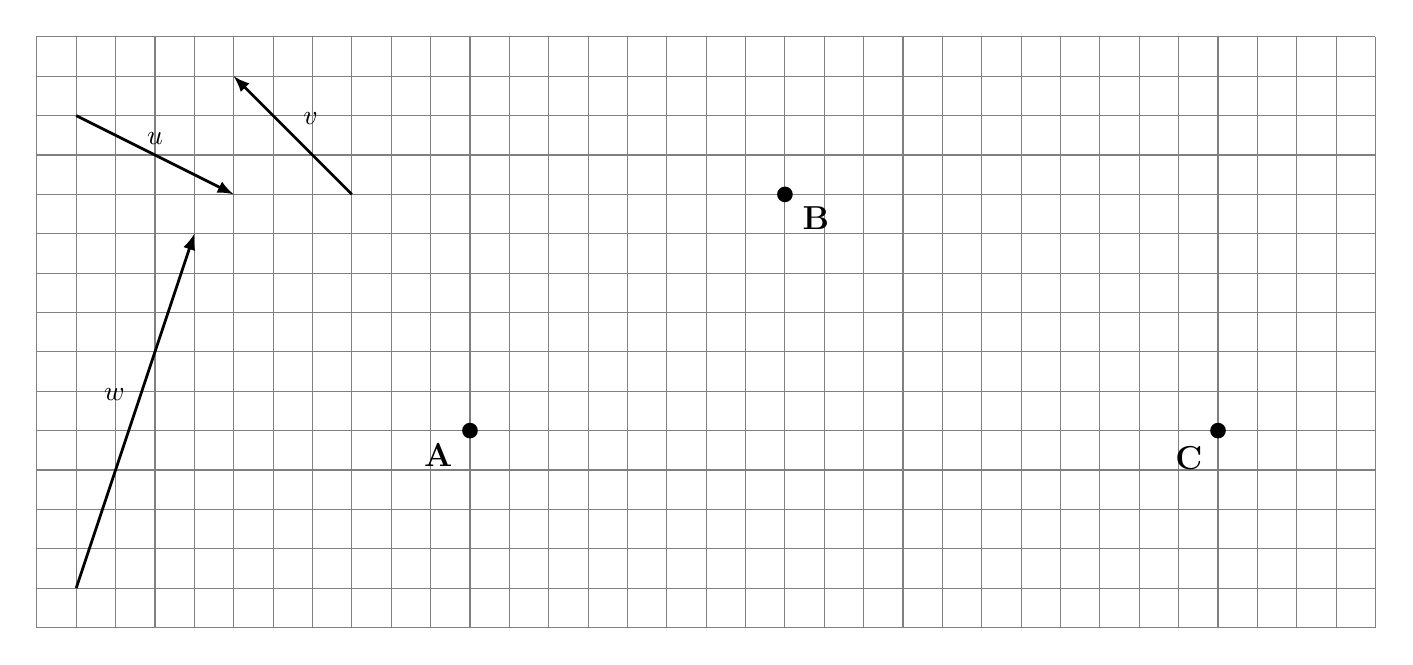
\begin{tikzpicture}[scale=0.5]
\node[draw=none] (liminf) at (-15,-7) {};
\node[draw=none] (limsup) at (19,8) {};
\draw[step=1,gray,thin] (liminf)+(-0.01,-0.01) grid (limsup)+(0.01,0.01);
\clip (liminf) rectangle (limsup);

\draw[line width=1pt,->,>=latex] (-14,6) -- ++(4,-2) node[pos=0.5,above] {$\vv u$};
\draw[line width=1pt,->,>=latex] (-7,4) -- ++(-3,3) node[pos=0.5,above right] {$\vv v$};
\draw[line width=1pt,<-,>=latex] (-11,3) -- ++(-3,-9) node[pos=0.5,above left] {$\vv w$};
\node[color=black,circle,minimum size=1pt,fill,inner sep=2pt,fill opacity=1,label={200:\textbf{\large A}}] (A) at (-4,-2) {};
\node[color=black,circle,minimum size=1pt,fill,inner sep=2pt,fill opacity=1,label={-20:\textbf{\large B}}] (B) at (4,4) {};
\node[color=black,circle,minimum size=1pt,fill,inner sep=2pt,fill opacity=1,label={-135:\textbf{\large C}}] (C) at (15,-2) {};
\end{tikzpicture}
\end{center}

\begin{enumerate}
\item Placer le point M tel que $\vv{AM}=\vv u+2 \vv v$
\item Placer le point N tel que $\vv{BN} = \vv{AB} - \vv w$
\item Placer le point O tel que $\vv{CO} = \vv v+\frac 1 2 \vv u+\frac 2 3 \vv w$
\item Placer le point I, milieu de $[AC]$.
\item Compléter: $\vv {AI} = \makebox[1cm]{\dotfill} \vv{AC}$
\end{enumerate}
\end{exercice}

\begin{exercice} \

\compo[0.7]
{
\quad En physique, un système est équilibré lorsque la somme des forces qui s'exercent sur lui est nulle.

\quad Le système représenté par les trois forces ci-contre est-il équilibré?

\points 2
}
{
\begin{center}
\vspace{-2.3cm}
\includegraphics[width=0.9\linewidth, trim=0 0 0 -1cm]{Forces DS NB.png}
\end{center}
}
\end{exercice}

\begin{exercice} \

\compo[0.65]
{\strut
On considère le triangle $ABC$, et les points $D \in [AB], E \in [AC]$ tels que $(DE) \parallel (BC)$, comme sur le schéma ci-contre.
\begin{enumerate}
\item Compléter: $\vv {AD} = \makebox[15mm]{\dotfill} \vv {AB}$, $\vv {AE} = \makebox[3cm]{\dotfill} $
\item Compléter puis justifier: $\vv {DE} = \makebox[3cm]{\dotfill} $
\end{enumerate}
\points 3
}
{
\begin{center}
%\vspace{-5mm}
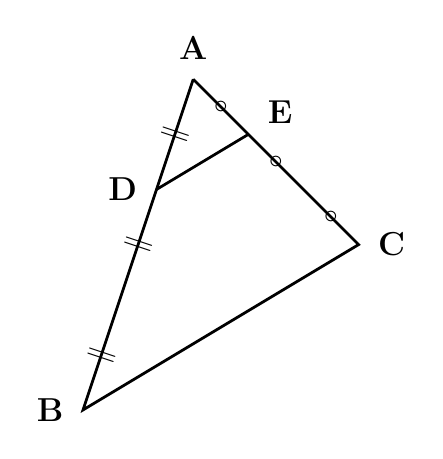
\begin{tikzpicture}[scale=0.7]
%\node[draw=none] (liminf) at (-10,-7.01) {};
%\node[draw=none] (limsup) at (10,7) {};
%\draw[step=1,gray,thin] (liminf) grid (limsup);
%\clip (liminf) rectangle (limsup);

\node[label={90:\textbf{\large A}}] (A) at (0,0) {};
\node[label={180:\textbf{\large B}}] (B) at (-2,-6) {};
\node[label={0:\textbf{\large C}}] (C) at (3,-3) {};
\node[label={180:\textbf{\large D}}] (D) at (-2/3,-2) {};
\node[label={5:\textbf{\large E}}] (E) at (1,-1) {};
\node (D') at (-4/3,-4) {};
\node (E') at (2,-2) {};
\path[draw=black,line width=1pt] (A.center) -- (B.center) -- (C.center) -- (A.center);

\newcommand{\barresa}[2]{\draw[draw=black,line width=1pt,decorate,decoration={markings, mark=at position .5  with {\node[transform shape] {$\parallel$};}}] (#1.center) -- (#2.center)}
\newcommand{\barresb}[2]{\draw[draw=black,line width=1pt,decorate,decoration={markings, mark=at position .5  with {\node[transform shape] {$\circ$};}}] (#1.center) -- (#2.center)}
\barresa A D;
\barresa D {D'};
\barresa {D'} B;
\barresb A E;
\barresb E {E'};
\barresb {E'} C;
\draw[line width=1pt] (D.center) -- (E.center);

\draw[line width=1pt,decorate,decoration={markings, mark=at position .5  with {\node[transform shape] {$\shortmid$};}}] (E.center) -- (C.center);
\draw[line width=1pt,decorate,decoration={markings, mark=at position .5  with {\node[transform shape] {$\shortmid$};}}] (D.center) -- (B.center);

\end{tikzpicture}
\end{center}
}
\end{exercice}

%%%%%%%%%%%%%%%%%%%%%%% Exercices inutilisés %%%%%%%%%%%%%%%%%%%%%%%

\begin{comment}

A évaluer:
\begin{itemize}
\item Vecteur
MM'
associé à la translation qui transforme M en M'. Direction, sens et
norme.
\item Égalité de deux vecteurs. Notation u. Vecteur nul.
\item Somme de deux vecteurs en lien avec l’enchaînement des translations. Relation de
Chasles.
\item Capacités
\begin{itemize}
\item Représenter géométriquement des vecteurs
\item Construire la somme de deux vecteurs
\end{itemize}
\end{itemize}

\begin{exercice} \

\compo[0.55]
{
Dans le repère ci-contre:
\begin{enumerate}
\item Tracer un vecteur $\vv v$ ayant la même longueur que $\vv u$, mais différent de $\vv u$.
\item Que dire du vecteur $\vv w$ par rapport au vecteur $\vv u$ ?
\end{enumerate}
\points 2
}
{
\begin{center}
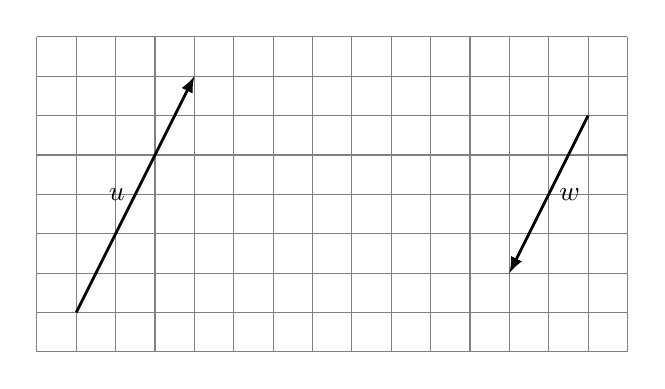
\begin{tikzpicture}[scale=0.5]
\node[draw=none] (liminf) at (0,0) {};
\node[draw=none] (limsup) at (15,8) {};
\draw[step=1,gray,thin] (liminf) grid (limsup);
\clip (liminf) rectangle (limsup);

\path [draw=black, line width=2pt] (0,0) -- (-1,-2) -- (0,-4);
%\node[draw=none] (A) at (1,1) {};
%\node[draw=none] (B) at (3,7) {};
\draw[line width=1pt,->,>=latex] (1,1) -- (4,7) node[pos=0.5,left] {$\vv u$};
\draw[line width=1pt,->,>=latex] (14,6) -- (12,2) node[pos=0.5,right] {$\vv w$};
\end{tikzpicture}
\end{center}
}
\end{exercice}

\begin{exercice} \ %Exo 2 original
\compo[0.38]
{
\begin{center}
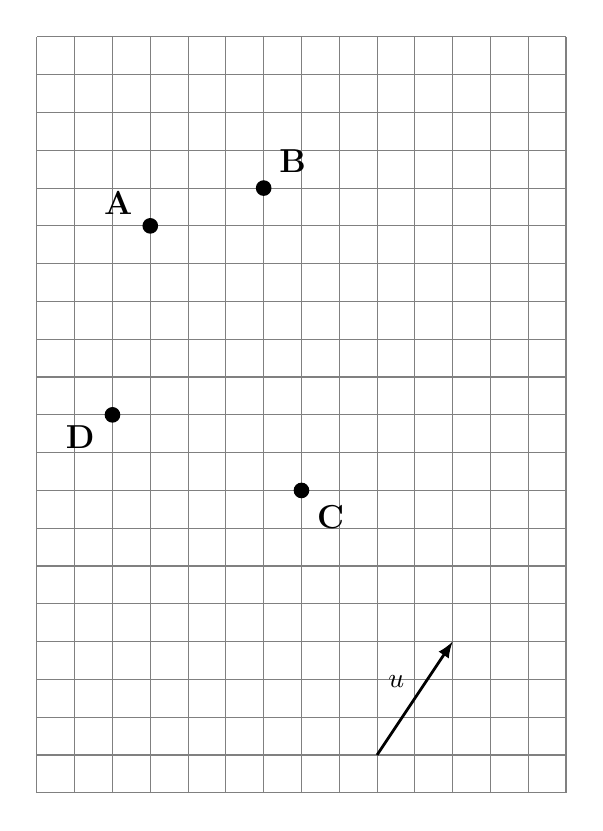
\begin{tikzpicture}[scale=0.48]
\node[draw=none] (liminf) at (0,-9.01) {};
\node[draw=none] (limsup) at (14,11) {};
\draw[step=1,gray,thin] (liminf) grid (limsup);
\clip (liminf) rectangle (limsup);

%\path [draw=black, line width=2pt] (0,0) -- (-1,-2) -- (0,-4);
%\draw[draw=black, fill = black, fill opacity = 0.3, line width=2pt, even odd rule] 
%        (-4,-8) rectangle (4,-4) (-3,-6.5) rectangle (-1,-5.5) (1,-6.5) rectangle (3,-5.5);
\node[color=black,circle,minimum size=1pt,fill,inner sep=2pt,fill opacity=1,label={170:\textbf{\large A}}] (A) at (3,6) {};
\node[color=black,circle,minimum size=1pt,fill,inner sep=2pt,fill opacity=1,label={45:\textbf{\large B}}] (B) at (6,7) {};
\node[color=black,circle,minimum size=1pt,fill,inner sep=2pt,fill opacity=1,label={-45:\textbf{\large C}}] (C) at (7,-1) {};
\node[color=black,circle,minimum size=1pt,fill,inner sep=2pt,fill opacity=1,label={190:\textbf{\large D}}] (D) at (2,1) {};
\draw[line width=1pt,->,>=latex] (9,-8) -- ++(2,3) node[pos=0.5,above left] {$\vv u$};
%\node[color=black,circle,minimum size=1pt,fill,inner sep=2pt,fill opacity=1,label={90:\textbf{\large E}}] (E) at (4,-4) {};
%\draw[line width=1pt, shorten <= -10cm, shorten >= -10cm] (A) -- (B);
\end{tikzpicture}
\end{center}
}
{
En utilisant le repère ci-contre:
\begin{enumerate}
\item Comparer trois caractéristiques des vecteurs $\vv u$ et $\vv {BD}$. \points 3
\item Tracer deux représentants du vecteur $\vv {AB}$, l'un d'origine $D$, l'autre d'extrémité $C$.
\item Placer $M$, l'image de $C$ par la translation de vecteur $\vv {DB}$.
\item Placer $N$, l'image de $C$ par la translation de vecteur $\vv {DC}$.
\item Quelle est la nature du quadrilatère $BCNM$? Justifier en utilisant des vecteurs: \points 3
\end{enumerate}
}
\end{exercice}

\end{comment}

\end{document}
